\section{Graph Algorithms}

	\begin{frame}
          \frametitle{Graphs}

          Pervasive data structure in Computer Science---an abstract
          representation in use to describe different domains, including
          trasport systems, electrical circuits, human interactions (social networks),
          computer networks, and software dependencies. \pause This class aims to
          discuss two concerns:   

          \vskip+1.5em

          \begin{itemize}
            \item graph representation 
            \item graph algorithms 
          \end{itemize}
        \end{frame}

\begin{frame}
\frametitle{Definition}

A graph $G$ is a pair $(V, E)$ where $V$ is an arbitrary
set and $E$ is a subset of $V^{(2)}$\pause---the set of all pairs of
elements in $V$.  The elements of $V$ are the {\color{blue}vertices} of the
graph, while the elements of $E$ are the {\color{blue}edges}
of the graph. 


\pause \vskip+1.5em
\begin{block}{Different flavors of graphs}

\begin{itemize}
\item directed graphs $\times$ undirected graphs
\item weighted graphs $\times$ unweighted graphs
\item ciclic graphs $\times$ aciclic graphs
\item \ldots
\end{itemize}
\end{block}
\end{frame}

\begin{frame}
\frametitle{Grapha representations}


\begin{itemize}
\item {\bf Adjacency-list:} compact representation recommended for
  {\color{blue}sparse graphs}  (where $|E|$ is smaller than 
  $|V|^{2}$). \pause 

\item {\bf Adjacency-matrix:} recommended for dense graphs or when we
  need to frequently search if an edge $(v_1, v_2)$ exists.   
\end{itemize}

\end{frame}

\begin{frame}
\frametitle{Samples (Fonte: Introduction to Algorithms)}
\centering{

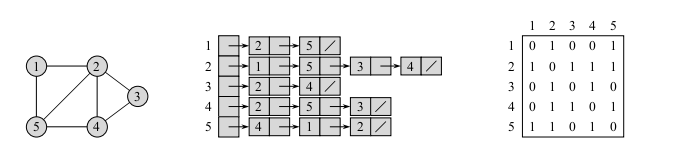
\includegraphics[scale=0.5]{images/undirected01.png}

\pause 

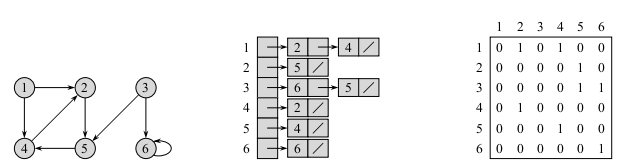
\includegraphics[scale=0.5]{images/directed01.png}	
}

\end{frame}


\begin{frame}
  \frametitle{Graph Algorithms}

  \begin{itemize}
   \item Search: Breadth-first search and Depth-first Search
   \item Single source shortest paths: Belkman-Ford and Dijkstra algorithms
   \item {\color{blue}Minimum Spanning Trees}
   \item {\color{blue}All-pairs shortest paths}  
  \end{itemize}
\end{frame}

\begin{frame}{Minimum Spanning Trees}

  Given a connected, weighted, and undirected graph $G = (V, E)$, we wish to
  find an acyclic subset $T \subseteq E$ that connects all of the vertices
  and whose {\color{blue}total} weight is minimized. \pause Since $T$ is acyclic and
  connects all of the vertices, it must form a (spanning) tree. 

  \pause \vskip+1.5em

  \centering{
    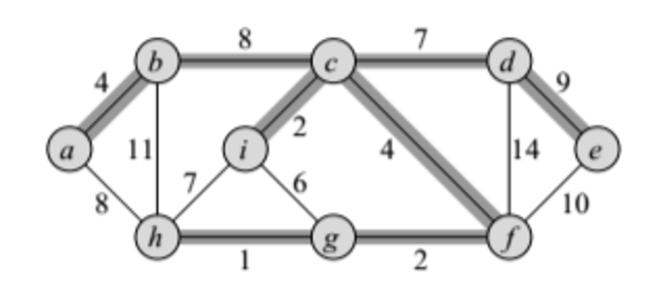
\includegraphics[scale=0.5]{images/st}
  }
\end{frame}


\begin{frame}

  The book presents an interesting description of the algortihms for
  Minimum Spanning Trees: a generic method for growing minimum spanning trees
  and two implementations of the algorithm (Kruskal's algorithm and Prim's algorithm).

  \pause \vskip+1.5em

  \begin{block}{Generic Method}
  \begin{algorithmic}
    \Procedure{Generic-MST}{G, w}
     \State $A = \emptyset$                 
     \While{$\text{A does not form a spanning tree}$}        
       \State $\text{find an edge (u, v) that is safe for A}$
       \State $A = A \cup \{(u, v)\}$
     \EndWhile
     \State {\bf return} $A$
    \EndProcedure
  \end{algorithmic}
  \end{block}

  \pause

  \begin{itemize}
    \item The challenge is to find out a {\color{blue}safe edge (u, v)}. 
  \end{itemize}
\end{frame}

\begin{frame}{Definitions}

  \begin{itemize}
   \item A {\color{blue}$cut(S, V-S)$} of an undirected graph $G = (V, E)$ is a partition of $V$. \pause 

   \item An {\color{blue}edge $(u, v) \in E$ crosses} a $cut(S, V-S)$ if one of its endpoints is in $S$ and
     the other is in $V-S$. \pause

   \item A {\color{blue}cut respects} a set A of edges if no edge in A crosses the cut. \pause
     
   \item An edge is a {\color{blue}light edge crossing} a cut if its weight is the minimum of any
     edge crossing the cut.  
  \end{itemize}
\end{frame}

\begin{frame}
  \begin{block}{Theorem}
    Given:
    \begin{itemize}
      \item $G = (V, E)$ is a connected, undirected graph
      \item $w : E \rightarrow R$ is a weighted function.
      \item $A$ is a subset of $E$ (included in some minimum spanning subtree for $G$)
      \item $(S, V-S)$ is any cut of $G$ that respects $A$
      \item $(u, v)$ is a light edge crossing $(S, V-S)$
    \end{itemize}
    then, edge $(u, v)$ is safe for $A$. 
  \end{block}

  Both algorithm implementations relie on this theorem. 
\end{frame}

\begin{frame}
  In the Kruskal's algorithm, the set $A$ is a {\color{blue}forest}
  whose vertices are all those of the given graph. The safe edge
  added to $A$ is allways a lest-weight edge in the graph that
  connects two distinct trees in the forest. \pause The book
  shows an implementation that benefits from the Disjoint Set
  data structure, whose interface contains three operations:
  \texttt{makeSet}, \texttt{findSet}, and \texttt{union}. 
\end{frame}

\begin{frame}
  \begin{small}
  \begin{algorithmic}
    \Procedure{MST-Kruskal}{G, w}
    \For{$\text{each vertex v } \in G.V$}
      \State $makeSet(v)$
    \EndFor
    \State $lst = \text{sort the edges of G.E into nondecreasing order by weight w}$
    \For{$(u, v) \rightarrow lst$}
      \If{$findSet(u) \neq findSet(v)$}
       \State $A = A \cup \{(u, v)\}$
       \State $union(u, v)$
      \EndIf 
    \EndFor
    \State {\bf return} $A$  
    \EndProcedure
  \end{algorithmic}
  \end{small}
\end{frame}

\begin{frame}{TODO}

  Study and implement the Prim's algorithm for
  computing minimum spanning trees. 
 
\end{frame}
